\section*{Question 5}
\subsection*{a)}
% How many process instances and events are in this event log? What is the median
% number of events in each trace and what is the average duration of them?
The process has 150370 cases and 561470 events. Median number of events is 5.
The average duration is 48.8 weeks.

\subsection*{b)}
% What will be the Disco process model for this event log when you set Activities
% slider to 80% and Paths slider to 10%? Interpret the (self-loop) edge from
% �Payment� to itself. How many times and for how many process instances this
% behavior happens?

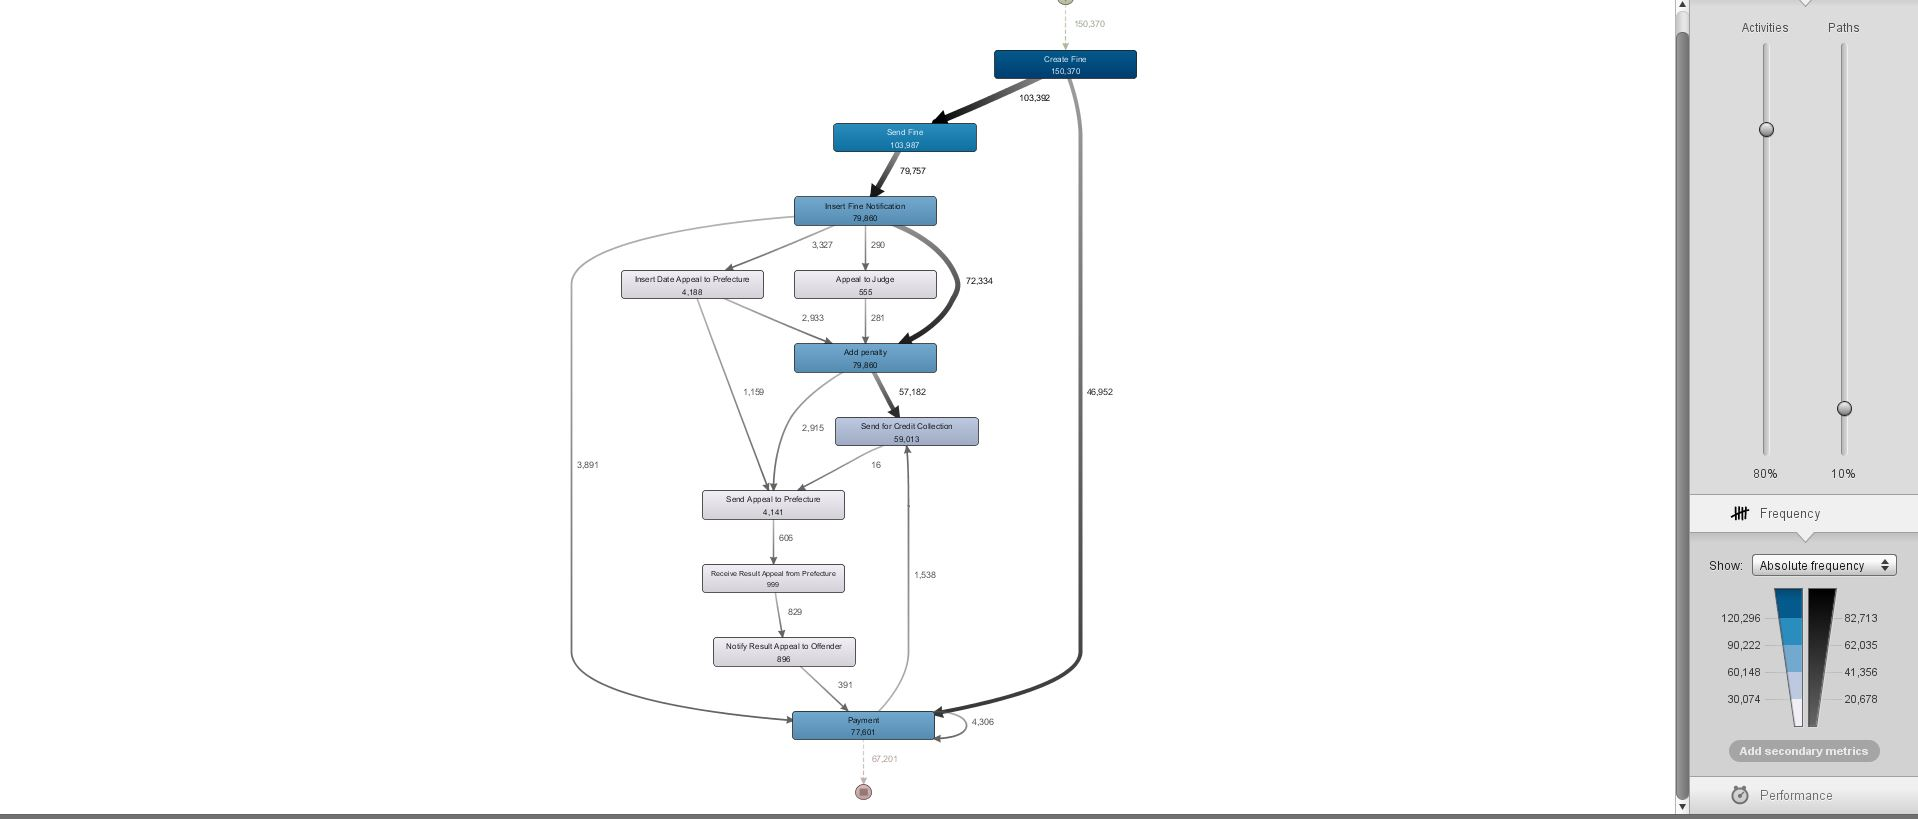
\includegraphics[width=0.8\textwidth]{Question5b.jpg}

The loop tells us, that a part of all people paid at least two times. If
you check the log data, you can see, that mostly it happens in the next 30 days.
Maybe they had a plan how to pay over weeks or had to pay penaltys.

This behavior happens 4306 and for 4014 cases. So there are cases, where it
happens more than one time. You also can see, that it happens at most 14 times.

\subsection*{c)}
%Using Disco, analyze the time distribution of events over the time covered by this
%log? What is your interpretation of the distribution of events over the time?
% Do you see any remarkable patterns in the distribution of events (drifts, repeating
%behavior, etc.)?
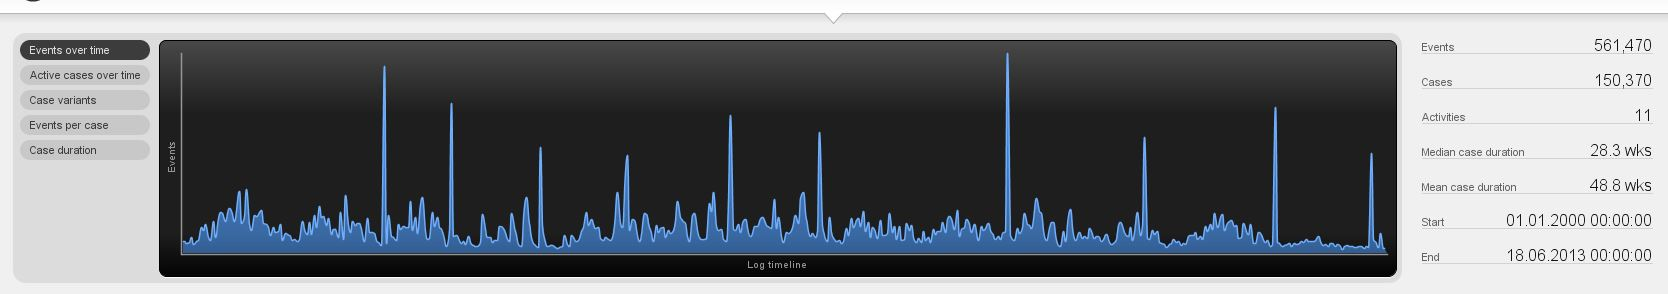
\includegraphics[width=0.8\textwidth]{Question5cDist.jpg}

You can see that the distribution is going up and down a little bit, but there
are 10 peaks to see where more happens. In the end activity gets
lower and the distance between the 6th and 7th peak is higher than between the
others.
It is always close to typical paydays, so maybe a lot of people then have
the money to pay the fine. It is also striking, that it is around the weekend.
Could be that there are more people riding too hard or just more people riding. 

The peakes are on:
06.04.2002 (Sa), 06.01.2003 (Mo), 05.01.2004 (Mo), 24.12.2004 (Fr), 20.02.2006 (Mo),
18.02.2007 (Su), 27.03.2009 (Fr), 08.10.2010 (Fr), 22.03.2012 (Thu), 19.04.2013
(Fr)

\subsection*{d)}
% How many variants are in this event log? What is the size (number of process
% instances) of the third most frequent variant? Also, explain what happens in this
% variant (report the sequence of activities).
There are 231 variants. The third most frequent variant has 20385 instances. It
just contains the behaviour \textbf{create} and \textbf{send fine}.

\subsection*{e)}
% Filter the event log using Disco while keeping 50% of the most common variants of
% process instances that finished until 01.01.2012 12: 12. What happens to the
% median and the average of case duration compared to the whole event log. Please
% also explain the difference between the median and the average (mean) of case
% duration.
It is just possible to $43\%$ or $56\%$. The average case duration shorts to
45.2 weeks from 48.8 weeks and the median to 20.9 weeks from 28.3 weeks in both
cases.
So the most common cases are in average faster finished than all cases in
average. This is like I would expect it.

The median is the instance in the middel. So if you write down all instances
sorted, it is the middel one. The average is the sum of all instances
divided by the number of instances. The average can change a lot for big or
extree small oultiers. The median shows more a real duration in the middle of
all instance durations.

\subsection*{f)}
% Discover the dotted chart view of the event log and interpret it using ProM. Adjust
% the Dotted chart settings in a way to answer question c. Are there any interesting
% (or odd) patterns in the dotted chart view that could explain the patterns found
% when answering question c?
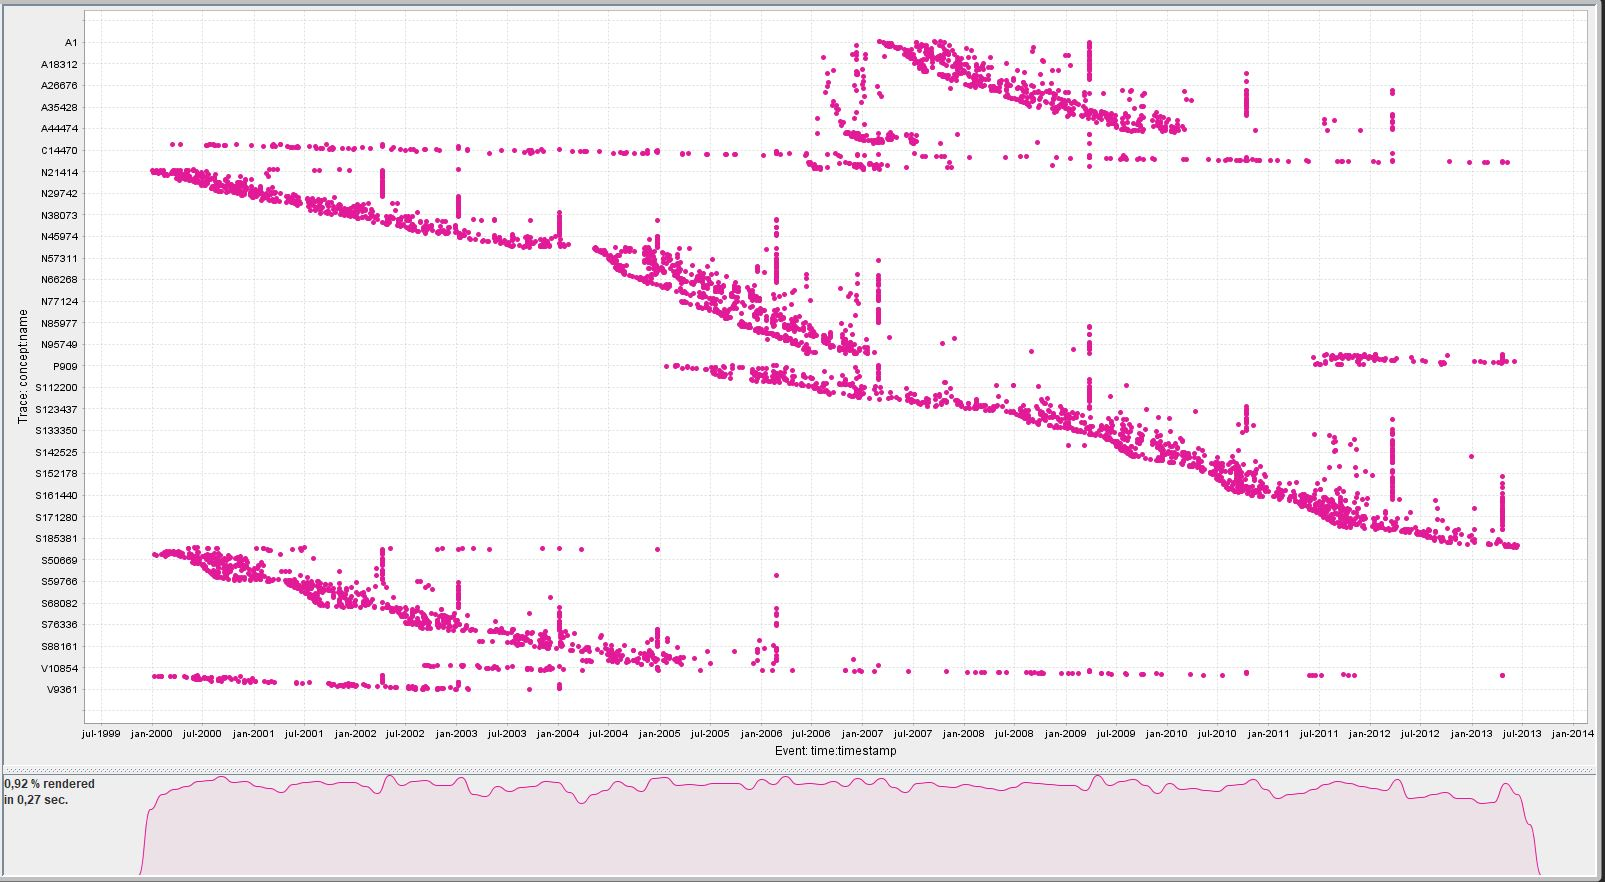
\includegraphics[width=\textwidth]{Question5f.jpg}

In the first dotted chart you see on what time which case is active.

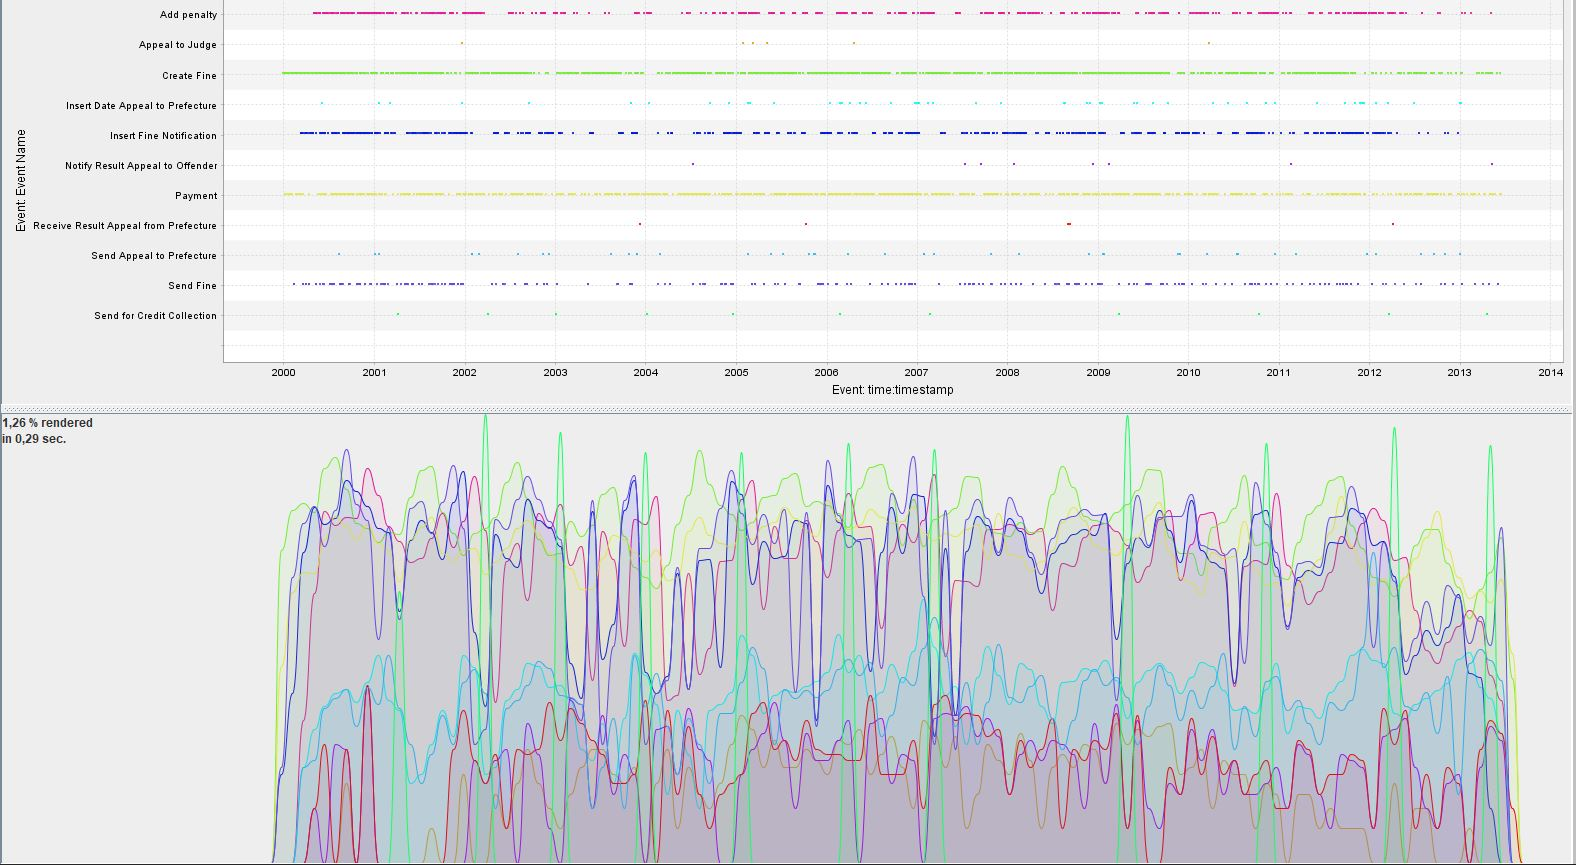
\includegraphics[width=\textwidth]{Question5fcZoomedIn.jpg}

For interpreting the dot chart for the question c) I changed the y-axis to the
event names so I can see when which events happen a lot and also coloured the
events.

For checking what exactly happens on the peaks I zoomed in (not to see in the
screenshot).

You can see that \textbf{Send for Credit Collection} is strongly connected to
the peakes to see in c). 

Payment happens close to always, but still it is a little bit bundled at the
peaks.

Furthermore I would say, that in disco it is more easy to see when peaks happen,
but in prom better to see what is happening on the peak days.

\subsection*{g)}
% Filter the event log using �filter log using simple heuristics� and then apply the
% Alpha algorithm (Alpha ++) on it. Filter the log appropriately. Show some insights
% that can only be seen after filtering.

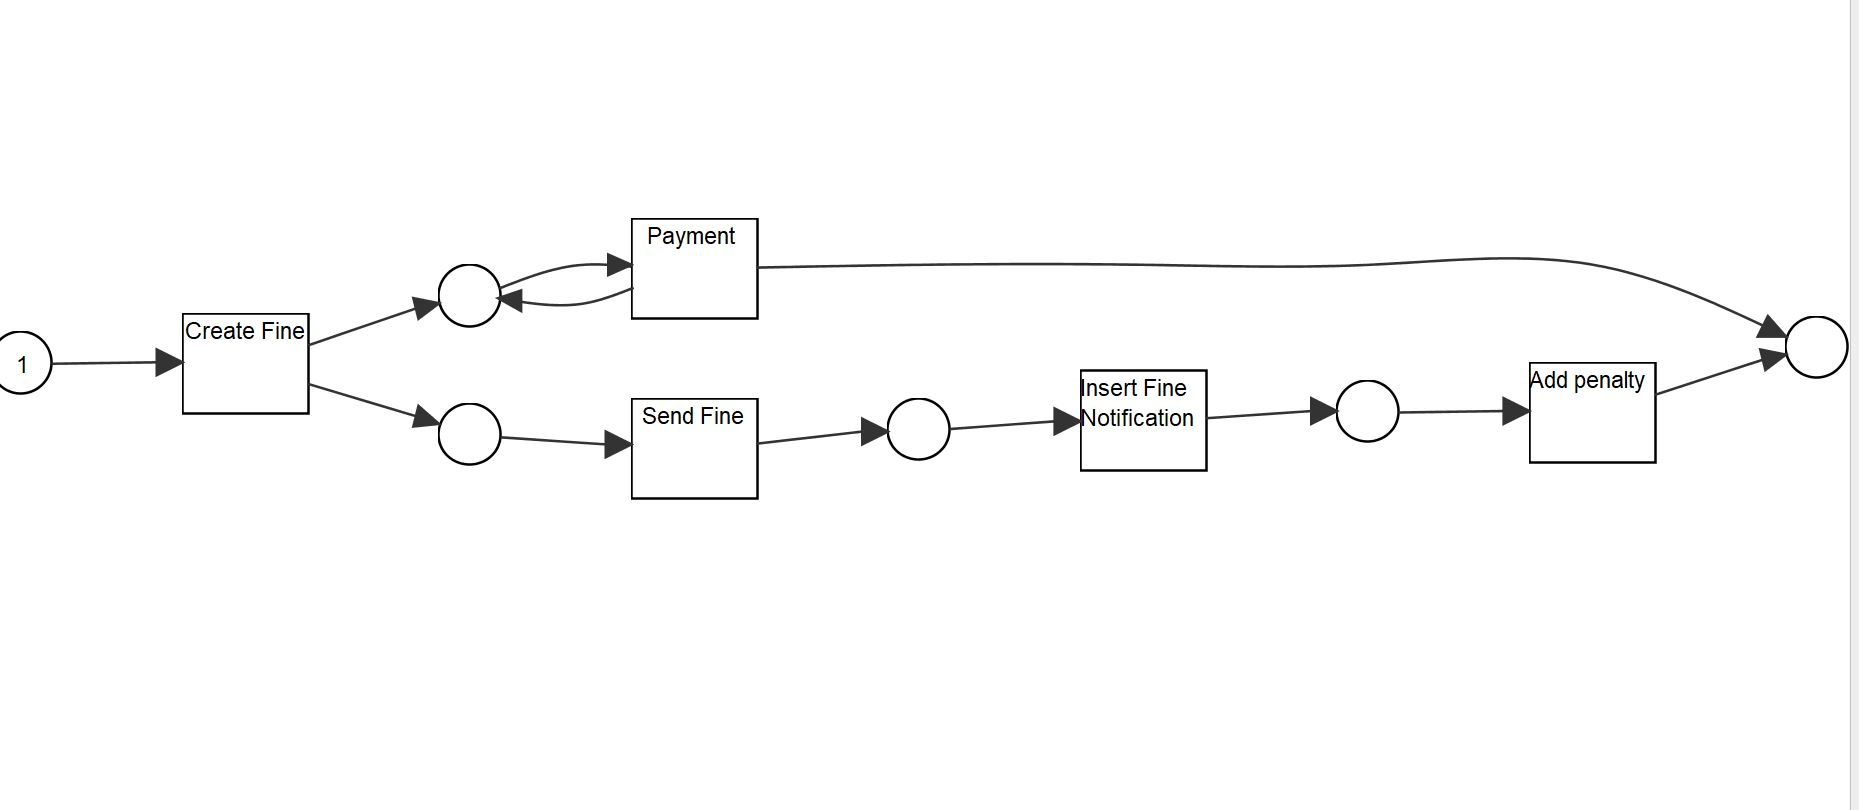
\includegraphics[width=\textwidth]{Question5g.jpg}

The filtering happened in the first case with basis settings. So 80\% of all
steps asked.
(2nd step log filter (end) just payment and send for credit, 3rd (event) add
penalty,create fine, insert fine notification, payment, send fine)

If you apply the alpha-algoirthm on the not filtered data you can not clearly
see in the resulting net, that the payment can happen always and also infinite
often. It sounds weird, because you do not expect someone paying before he gets
the fine, but looking at the data it happens.

I also filtered with different settings(, but did not have enough insights
about the data)
\begin{enumerate}
  \item 90\% for create fine and complete and choosing all end events with 80\%
  and including all events with 80\%\\
  \item 50\% for create fine+complete rest like basis\\
  \item and a few more not safed
\end{enumerate}

The alpha-algorithm used for this different setting does not give more
insights, so I does not include screenshots of it. (The data is foundable in my
filesystem)

\subsection*{h)}
% Use the filtered event log in the previous question and this time use it as input for
% Disco. Which parts of the process are time consuming for most of the process
% instances? Answer this by interpreting the Disco model.

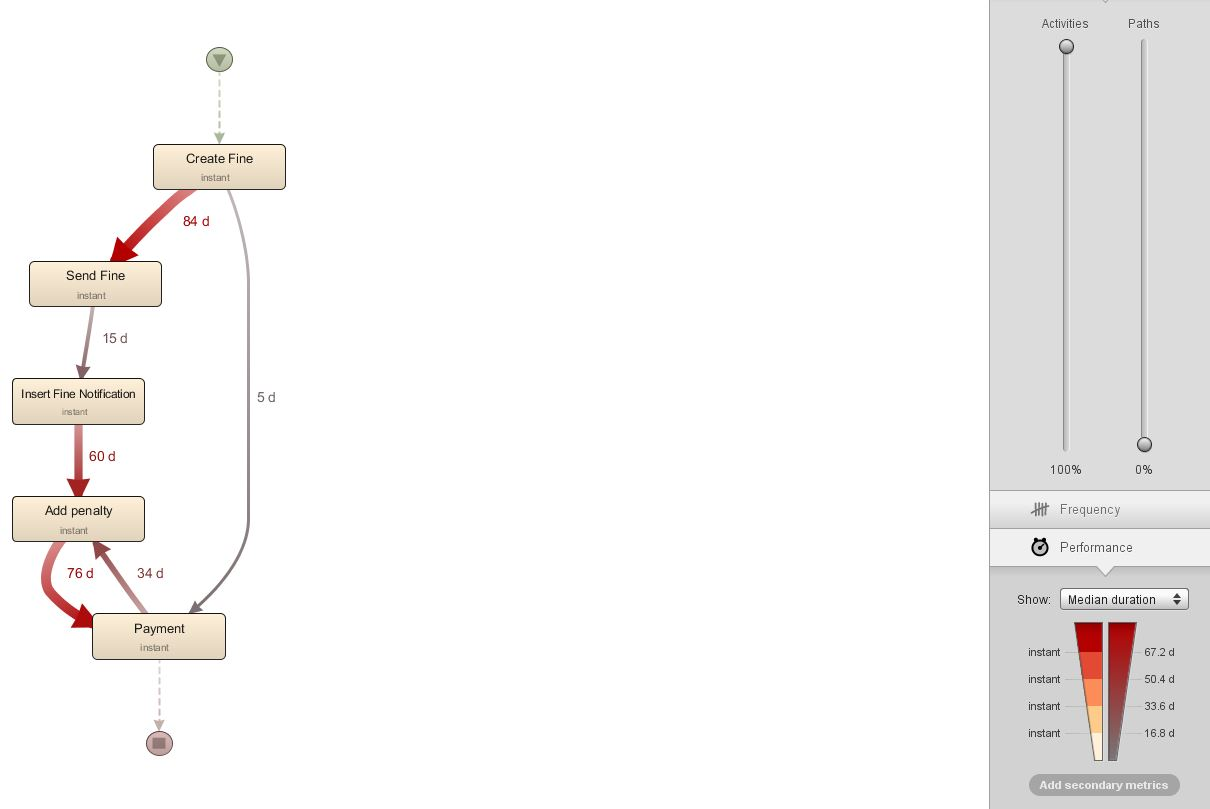
\includegraphics[width=\textwidth]{Question5h.jpg}

84days is the median for send fine. I chose the median, because then you get a
better idea what happens most of the times, because it is less exposed to
outliers.
(The biggest mean is 23.3 weeks between add penalty and payment.)

Additionaly you can see, that after exactly 60days the penalty gets
added.
